% This file should be replaced with your file with thesis content.
%=========================================================================
% Authors: Michal Bidlo, Bohuslav Křena, Jaroslav Dytrych, Petr Veigend and Adam Herout 2019

% For compilation piecewise (see projekt.tex), it is necessary to uncomment it and change
% \documentclass[../projekt.tex]{subfiles}
% \begin{document}

\chapter{Note to the reader}
Through the thesis, the expression "iff" refers to "if and only if".

\chapter{Introduction}
\todo{Add motivation for thesis, talk about importance of optics simulations, talk about uses, show examples. Talk about the need to compare simulation software.}

\chapter{Review of computational electromagnetics and compilers}
This chapter aims to give the reader a broad understanding of the subjects of matter. It provides an overview of the physics behind the aforementioned simulations and an introduction to the basic concepts of compiler design and the underlying formal languages. This chapter will not delve into the specifics of each subject at hand but will provide the reader with the foundations necessary to comprehend the rest of this thesis.

\section{Computational Electromagnetics}
\subsection*{Maxwell's equations}
\subsubsection*{Curl theorem}
\subsubsection*{Divergence theorem}
\paragraph{Magnetic monopoles}

\subsection*{Finite Difference Time Domain}
\subsection*{Mie Scattering}
\section{Formal Languages}


\begin{definition}[Alphabet]
\label{def:alphabet}
Let $\Sigma$ be an \emph{alphabet}, a finite nonempty set of symbols. Then $\Sigma ^{*}$ defines the set of all sequences $w$:
$$w= a_1 a_2 a_3 \dots a_{n-1} a_n, a_i \in \Sigma \text{ for } i \in \mathbb{N}$$
\end{definition}

The sequence symbols $w$ is called a \emph{word}. The length of a word is $|w| = n$. The word with a length of 0 is called an \emph{empty word} denoted as $\lambda$.

\begin{definition}[Language]
\label{def:language}
The set $L$ where $L\subseteq \Sigma^{*}$ is know as the formal language over the alphabet $\Sigma$. 
\end{definition}
The words $L = \left\lbrace \lambda, a, b, aa, ab, bb \right\rbrace$ are some words of a language $L$ over the alphabet $\Sigma=\left\lbrace a,b \right\rbrace$.
Other examples for languages over the alphabet $\Sigma=\left\lbrace a,b \right\rbrace$ might include:
\begin{itemize}

\item $L_1 = \left\lbrace \lambda \right\rbrace$
\item $L_2 = \left\lbrace a \right\rbrace$
\item $L_3 = \left\lbrace aaa \right\rbrace$
\item $L_4 = \left\lbrace a^i,b^i; i \in \mathbb{N} \right\rbrace$
\end{itemize}



\begin{samepage}
\begin{large}
\textbf{Notation conventions}
\end{large}

\begin{itemize}
\item Iteration
Let $a^i; a \in \Sigma \text{and} i \in \mathbb{Z}$ be the iteration of a character $a$, where $|a^i| = i$.
Examples bellow.
\begin{itemize}
\item $a^0 = \lambda$
\item $a^1 = a$
\item $a^2 = aa$
\item $a^i = a_0 a_1 a_2 \dots a_i; i \in \mathbb{N}$
\end{itemize}


\item Concatenation
Let $w \cdot w^{'}; w, w^{'} \in \Sigma^{*}$ be the concatenation of the words $w$ and $w^{'}$.

$w = a_1 a_2 a_3 \dots a_n ; w^{'} = a^{'}_1 a^{'}_2 a^{'}_3 \dots a^{'}_m; n,m \in \mathbb{Z}$ then

$w\cdot w^{'} = w w^{'} = a_1 a_2 a_3 \dots a_n a^{'}_1 a^{'}_2 a^{'}_3 \dots a^{'}_m$
\item \todo{Kleene star}
\end{itemize}
\end{samepage}

Languages are often defined by grammars.
\begin{definition}[Grammar]
\label{def:grammar}
\cite{formal_languages}
Let an ordered quadruple $G$ define a grammar such that: $G=\left(N, \Sigma, P, S \right)$, where:
\begin{enumerate}
\item $N$ is a finite set of \emph{nonternminal} symbols
\item $\Sigma$ is an alphabet finite set of \emph{terminal} symbols, such that $N \cap \Sigma = \varnothing$
\item $P$ is a finite set of rewriting rules known as \emph{productions}, ordered pairs $\left( \alpha, \beta \right)$.
$P$ is a subset of the cartesian product of $\alpha = \left(N \cup \Sigma\right)^* N \left(N \cup \Sigma\right)^*$ and $\beta = \left(N \cup \Sigma\right)^*$


Productions are denoted as $\alpha \rightarrow \beta$.
If there are multiple productions with the same left hand side ($\alpha$), we can group their right hand sides ($\beta$).


$\alpha \rightarrow \beta_1, \alpha \rightarrow \beta_2$ may be written as $\alpha \rightarrow \beta_1 | \beta_2$

\item $S$ is the starting symbol of the grammar $G$, where $S \in N$
\end{enumerate}
\end{definition}

Productions $\alpha \rightarrow \beta$ symbolize, that given the words $V,W,x,y \in \left( N \cup \Sigma \right)^{*}$, the word $V$ can be rewritten as follows:
$V \Rightarrow W$ iff there are words, which satisfy the following condition, $V=x\alpha y \wedge W=x\beta y$ and $\alpha \rightarrow \beta \in P$.

\begin{definition}[Derivation]
\label{def:derivation}
$V \stackrel{*}{\Rightarrow}  W$ iff there is a finite set of words 
$$ v_0, v_1, v_2, \dots, v_z;\medskip z \in \mathbb{Z}$$
such that $v_0 = V$ and $v_z = W$ where each is rewritten from the previous word. Such a sequence of applications of productions is called a derivation.
The length of a derivation is given by $z$. 
\end{definition}




\section{Compilers}


Compilers are complex algorithms, \emph{programs}, that translate a human readable input known as \emph{source code} into a representation more suitable for computers to run. The introduction of compilers 


Today's world undeniably relies on software more than ever before. It is imperative for developers to be able to efficiently write software. Software today is written in programming languages, high-level human-readable notations for defining how a program should run. However, before a program can be run on a system, it has to be translated (or \emph{compiled}) into low-level machine code, which computers can run. The computer program that facilitates this translation is called a \emph{compiler}. See \ref{fig:compiler}.

\begin{figure}
  \caption{Figure describing the compiler as a single unit.}
  \label{fig:compiler}
  \centering
  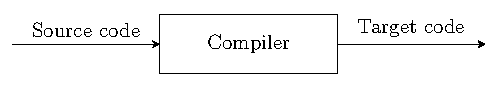
\includegraphics[width=0.75\textwidth]{figures/compiler.pdf}
\end{figure}



Compilers are complex programs. It is helpful to break them down into parts, each handling different tasks, which are chained together to form a compiler. Modern compilers are composed of many phases, such as the \emph{Lexical Analyzer}, \emph{Syntax Analyzer}, \emph{Semantic Analyzer}, \emph{Intermediate Code Generator}, \emph{Machine-Independent Code Optimizer}, \emph{Code Generator}, \emph{Machine-Dependent Code Optimizer} \cite{dragon}, however this chapter covers the components relevant to this thesis. See relevant stages in \ref{fig:compiler-stages}.


\begin{figure}
  \caption{Figure describing the compiler stages.}
  \label{fig:compiler-stages}
  \centering
  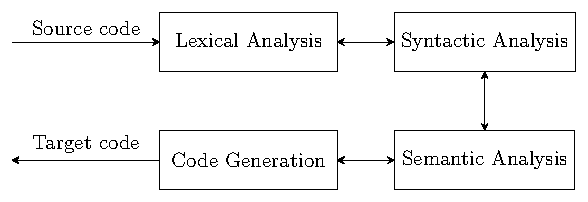
\includegraphics[width=0.75\textwidth]{figures/compiler-stages.pdf}
\end{figure}

\subsection*{Lexical Analysis}
The first stage of a compiler is lexical analysis, also known as a \emph{lexer} or \emph{tokenizer}. For the remainder of this thesis, \emph{lexer} will refer to the lexical analysis stage of a compiler. The lexer consumes a stream of characters, the \emph{source code}, and returns a stream of \emph{tokens}. A \emph{token} is a lexically indivisible unit, for example, the Python keyword \texttt{return}, you cannot divide it further, for example, into \texttt{re} \texttt{turn}. Each token is comprised of characters. The rule that defines which combination of characters constitutes a given token is called a \emph{pattern}. The sequence of characters matching a pattern is called a \emph{lexeme}, the \emph{lexeme} is stored along with the token as a value.

%Lexical analysis may be further divided into two distinct stages, however they are often implemented together. These stages are the \emph{scanner} and \emph{evaluator}.


\subsection*{Regular Expressions}
A compact way to represent the patterns accepting tokens are \emph{regular expressions}. Regular expressions are an algebraic definition of patterns, they specify \emph{regular languages}, $\mathcal{L}_3$


\subsection*{Formal grammars}
\subsection*{LL parsing}


\chapter{Transpiler implementation}
\todo{mention lexer regex implementation}
\todo{mention LL table calculation according to theory}
\todo{write about transformation of ast}


\chapter{Evaluation of results}
\todo{talk about methodology}
\todo{test examples analyticall vs FDTD}
\chapter{Conclusion}
\todo{compare lumerical and meep}
\todo{test result TBD}




%=========================================================================

% For compilation piecewise (see projekt.tex), it is necessary to uncomment it
% \end{document}